% Template for Elsevier CRC journal article
% version 1.2 dated 09 May 2011

% This file (c) 2009-2011 Elsevier Ltd.  Modifications may be freely made,
% provided the edited file is saved under a different name

% This file contains modifications for Transportation Research Procedia

% Changes since version 1.1
% - added "procedia" option compliant with ecrc.sty version 1.2a
%   (makes the layout approximately the same as the Word CRC template)
% - added example for generating copyright line in abstract

%-----------------------------------------------------------------------------------

%% This template uses the elsarticle.cls document class and the extension package ecrc.sty
%% For full documentation on usage of elsarticle.cls, consult the documentation "elsdoc.pdf"
%% Further resources available at http://www.elsevier.com/latex

%-----------------------------------------------------------------------------------

%%%%%%%%%%%%%%%%%%%%%%%%%%%%%%%%%%%%%%%%%%%%%%%%%%%%%%%%%%%%%%
%%%%%%%%%%%%%%%%%%%%%%%%%%%%%%%%%%%%%%%%%%%%%%%%%%%%%%%%%%%%%%
%%                                                          %%
%% Important note on usage                                  %%
%% -----------------------                                  %%
%% This file should normally be compiled with PDFLaTeX      %%
%% Using standard LaTeX should work but may produce clashes %%
%%                                                          %%
%%%%%%%%%%%%%%%%%%%%%%%%%%%%%%%%%%%%%%%%%%%%%%%%%%%%%%%%%%%%%%
%%%%%%%%%%%%%%%%%%%%%%%%%%%%%%%%%%%%%%%%%%%%%%%%%%%%%%%%%%%%%%

%% The '3p' and 'times' class options of elsarticle are used for Elsevier CRC
%% The 'procedia' option causes ecrc to approximate to the Word template
\documentclass[3p,times,procedia]{elsarticle}
\flushbottom

%% The `ecrc' package must be called to make the CRC functionality available
\usepackage{ecrc}
%\usepackage{amsmath}


%% The ecrc package defines commands needed for running heads and logos.
%% For running heads, you can set the journal name, the volume, the starting page and the authors

%% set the volume if you know. Otherwise `00'
\volume{00}

%% set the starting page if not 1
\firstpage{1}

%% Give the name of the journal
\journalname{Transportation Research Procedia}

%% Give the author list to appear in the running head
%% Example \runauth{C.V. Radhakrishnan et al.}
\runauth{Lucas Javaudin}

%% The choice of journal logo is determined by the \jid and \jnltitlelogo commands.
%% A user-supplied logo with the name <\jid>logo.pdf will be inserted if present.
%% e.g. if \jid{yspmi} the system will look for a file yspmilogo.pdf
%% Otherwise the content of \jnltitlelogo will be set between horizontal lines as a default logo

%% Give the abbreviation of the Journal.
\jid{trpro}

%% Give a short journal name for the dummy logo (if needed)
%\jnltitlelogo{Transportation Research}

%% Hereafter the template follows `elsarticle'.
%% For more details see the existing template files elsarticle-template-harv.tex and elsarticle-template-num.tex.

%% Elsevier CRC generally uses a numbered reference style
%% For this, the conventions of elsarticle-template-num.tex should be followed (included below)
%% If using BibTeX, use the style file elsarticle-num.bst

%% End of ecrc-specific commands
%%%%%%%%%%%%%%%%%%%%%%%%%%%%%%%%%%%%%%%%%%%%%%%%%%%%%%%%%%%%%%%%%%%%%%%%%%

%% The amssymb package provides various useful mathematical symbols

\usepackage{amssymb}
%% The amsthm package provides extended theorem environments
%% \usepackage{amsthm}

%% The lineno packages adds line numbers. Start line numbering with
%% \begin{linenumbers}, end it with \end{linenumbers}. Or switch it on
%% for the whole article with \linenumbers after \end{frontmatter}.
%% \usepackage{lineno}

%% natbib.sty is loaded by default. However, natbib options can be
%% provided with \biboptions{...} command. Following options are
%% valid:

%%   round  -  round parentheses are used (default)
%%   square -  square brackets are used   [option]
%%   curly  -  curly braces are used      {option}
%%   angle  -  angle brackets are used    <option>
%%   semicolon  -  multiple citations separated by semi-colon
%%   colon  - same as semicolon, an earlier confusion
%%   comma  -  separated by comma
%%   numbers-  selects numerical citations
%%   super  -  numerical citations as superscripts
%%   sort   -  sorts multiple citations according to order in ref. list
%%   sort&compress   -  like sort, but also compresses numerical citations
%%   compress - compresses without sorting
%%
\biboptions{authoryear}

% \biboptions{}

% if you have landscape tables
\usepackage[figuresright]{rotating}
%\usepackage{harvard}
% put your own definitions here:x
%   \newcommand{\cZ}{\cal{Z}}
%   \newtheorem{def}{Definition}[section]
%   ...

% add words to TeX's hyphenation exception list
%\hyphenation{author another created financial paper re-commend-ed Post-Script}

% declarations for front matter

\usepackage[bookmarks=false]{hyperref}
    \hypersetup{colorlinks,
      linkcolor=blue,
      citecolor=blue,
      urlcolor=blue}

\usepackage{siunitx}

\usepackage{etoolbox}
\renewcommand{\bfseries}{\fontseries{b}\selectfont}
\robustify\bfseries
\newrobustcmd{\B}{\bfseries}

\begin{document}
\begin{frontmatter}

%% Title, authors and addresses

%% use the tnoteref command within \title for footnotes;
%% use the tnotetext command for the associated footnote;
%% use the fnref command within \author or \address for footnotes;
%% use the fntext command for the associated footnote;
%% use the corref command within \author for corresponding author footnotes;
%% use the cortext command for the associated footnote;
%% use the ead command for the email address,
%% and the form \ead[url] for the home page:
%%
%% \title{Title\tnoteref{label1}}
%% \tnotetext[label1]{}
%% \author{Name\corref{cor1}\fnref{label2}}
%% \ead{email address}
%% \ead[url]{home page}
%% \fntext[label2]{}
%% \cortext[cor1]{}
%% \address{Address\fnref{label3}}
%% \fntext[label3]{}

\dochead{World Conference of Transport Research, Toulouse 2026 (WCTR 2026 Toulouse)}%

\title{Aggregating Mobility Surveys to Understand Intermodality: Evidence from 78 French Surveys}

%% use optional labels to link authors explicitly to addresses:
%% \author[label1,label2]{<author name>}
%% \address[label1]{<address>}
%% \address[label2]{<address>}



\author[cyu,lvmt]{Lucas Javaudin\corref{cor1}}

\address[cyu]{THEMA, CY Cergy Paris Université, 33 Boulevard du Port, 95000 Cergy, France}
\address[lvmt]{LVMT, ENPC, Institut Polytechnique de Paris, Univ Gustave Eiffel, 6-8 Avenue Blaise Pascal, 77420 Champs-sur-Marne, France}

\begin{abstract}
%% Text of abstract
    Intermodality refers to the combination of multiple transportation modes during a single trip.
    It can help reduce carbon emissions, especially in rural and peri-urban areas where public transit can be hard to reach by walking.
    Yet, since only about \SI{1}{\%} of trips in France are intermodal, studying this behavior is difficult.
    This study introduces MobiSurvStd, an open-source tool that standardizes French mobility survey data.
    With this tool, I combine data from 78 surveys conducted between 2008 and 2022 to build a detailed dataset representing travel patterns across France.
    The analysis shows that most intermodal trips combine car use with public transit.
    In these trips, the public-transit segment is about 3 times longer than the car segment.
    Trips that start by car and continue with public transit often link outer areas to city centers, with trains and coaches being the most common transit mode used to access the network.
    The final part of this study links survey data with the actual locations of public-transit stops to test whether travelers choose the closest train station to their departure point.
    The results offer insights for transportation planners aiming to design multimodal hubs that make sustainable intermodal travel more convenient.
\end{abstract}

\begin{keyword}
    intermodality; mobility surveys; survey standardization; park-and-ride


%% keywords here, in the form: keyword \sep keyword

%% PACS codes here, in the form: \PACS code \sep code

%% MSC codes here, in the form: \MSC code \sep code
%% or \MSC[2008] code \sep code (2000 is the default)

\end{keyword}
\cortext[cor1]{Corresponding author.}
\end{frontmatter}

%\correspondingauthor[*]{Corresponding author. Tel.: +0-000-000-0000 ; fax: +0-000-000-0000.}
\email{lucas.javaudin@enpc.fr}

\vspace{-2em}
\section*{Highlights}
\begin{itemize}
    \item An open-source tool, MobiSurvStd, is introduced to standardize and aggregate 78 French mobility surveys (2008–2022). This harmonized dataset, representing over two million trips, enables national-scale analysis of intermodality and other rare travel behaviors previously difficult to study due to fragmented survey formats.
    \item Results reveal that \SI{85}{\%} of intermodal trips combine car and public transit, with cars mainly serving as access modes to the network. On average, the public-transit segment covers three times the distance of the car segment, and these trips typically connect rural or suburban origins to city centers.
    \item A novel spatial analysis links survey data with transit-stop locations to examine whether travelers use their nearest stop. Findings show proximity strongly drives train access choices, while tram and metro users often prioritize other factors, such as service quality and connectivity, over distance.
\end{itemize}


%%
%% Start line numbering here if you want
%%
% \linenumbers

%% main text
%\vspace*{-12pt}
%\enlargethispage{-7mm}
\section{Introduction}
\label{sec:introduction}

Intermodality designates a transportation strategy where travelers combine multiple modes within a single journey.
This approach offers efficiency advantages by allowing travelers to select the most appropriate mode for each sgement of their trip.
For example, travelers might use private vehicles in low-density areas where roads are uncongested, switch to public transit in dense urban centers with frequent service, and opt for bicycles in congested urban areas.

Beyond improving travel efficiency, intermodality presents environmental benefits, particularly in low-density areas with poor public-transit coverage.
Rather than completing entire journeys by car, travelers can use their car only as access mode to nearby public-transit stops, then continue the majority of their trip using more sustainable public-transit options.
This modal combination can reduce considerably the overall carbon footprint of the journey, without increasing significantly travel time.

The potential of intermodality is particularly relevant in France, where the Service Express Régional Métropolitain (SERM) initiative aims to develop multimodal transportation hubs in peripheral and low-density areas.
Well-served transit hubs would be created in rural and suburban locations, where private vehicles could efficiently connect travelers to these hubs.

Mobility surveys, commonly referred to as household travel surveys, serve as essential data sources for examining individual and household travel behaviors, including intermodal transportation patterns.
These surveys support diverse research applications across the transportation field.
For example, \citet{Ghimire2024} use the U.S. National Household Travel Survey to investigate the use of walking and cycling among low-income households.
\citet{Durand2016} analyze data from the California Household Travel Survey to explore the relationship between trip distance and walking access to public transit.
\citet{Poulhes2021} employ the Paris regional survey to quantify health benefits associated with the city's Low Emission Zone.

Comprehensive analyses of intermodality behavior remain limited in the existing literature.
Previous research has typically focused on specific aspects of intermodal travel: the combination of bicycle and public transit \citep{Kapuku2024}, the propensity to travel by park-and-ride \citep{Huang2021}, or the choice of park-and-ride facilities \citep{Webb2020,Irawati2022}.

Given the relative rarity of intermodal trips, which account for about \SI{1}{\%} of all trips in France, aggregating data from multiple mobility surveys becomes essential to obtain sufficient observations for statistically robust analysis.
To address the challenges posed by fragmented mobility survey data in France, this study introduces MobiSurvStd, an open-source library specifically designed to standardize French mobility survey data.

While \citet{Wittwer2018} developed a methodology for harmonizing mobility surveys across five European cities, this study represents, to the best of our knowledge, the first comprehensive attempt to systematically harmonize and aggregate regional mobility surveys at a national scale.
This research thus fills a gap in the literature by providing a tool that enables two types of analysis.
First, it facilitates the study of less prevalent travel behaviors, such as intermodality, that require large, aggregated datasets from multiple surveys to achieve statistical significance.
Second, it provides the capacity to examine variations in travel behavior across regions and time periods.

Using the MobiSurvStd library, we construct a comprehensive dataset comprising 78 mobility surveys conducted between 2008 and 2022 in France, covering approximately \num{787000} individuals and 2.11 million trips.
Leveraging this extensive dataset, our research aims to examine the characteristics, patterns, and determinants of intermodal trips in France.
We place particular emphasis on the spatial dimensions of intermodality, investigating the influence of urban density and access to transit infrastructure.
The main part of our analysis focuses on trips combining public transit and car, which constitutes about \SI{85}{\%} of all intermodal trips.

\section{Standardization of Mobility Surveys}

In France, mobility surveys are conducted by multiple institutions, each using distinct formats and methodologies.
Most surveys are administered by the CEREMA organization, for both urban and rural territories.
In the Paris region, however, surveys are managed by \emph{Île-de-France Mobilités}, the local transport authority, through the \citet{EGT2010}, which is conducted approximately once per decade.
The Ministry of Ecology also carries out surveys at the national level, with the most recent one, the \emph{Enquête Mobilité des Personnes}, which was conducted in 2019.

Efforts to standardize these surveys have been made, including CEREMA's introduction of the EMC\textsuperscript{2} format in 2018 (e.g., \citealp{EMC2Marseille}).
Before this standardization, however, CEREMA surveys used a variety of formats: EMD (e.g., \citealp{EMDNice}), EDGT (e.g., \citealp{EDGTLyon}), and EDVM (e.g., \citealp{EDVMCreil}).
The absence of a unified framework complicates efforts to compare surveys across different regions or time periods.
Figure~\ref{fig:survey_map} presents a geographical overview of 78 local mobility surveys conducted in France between 2008 and 2022.

\begin{figure}[htpb]
    \centering
    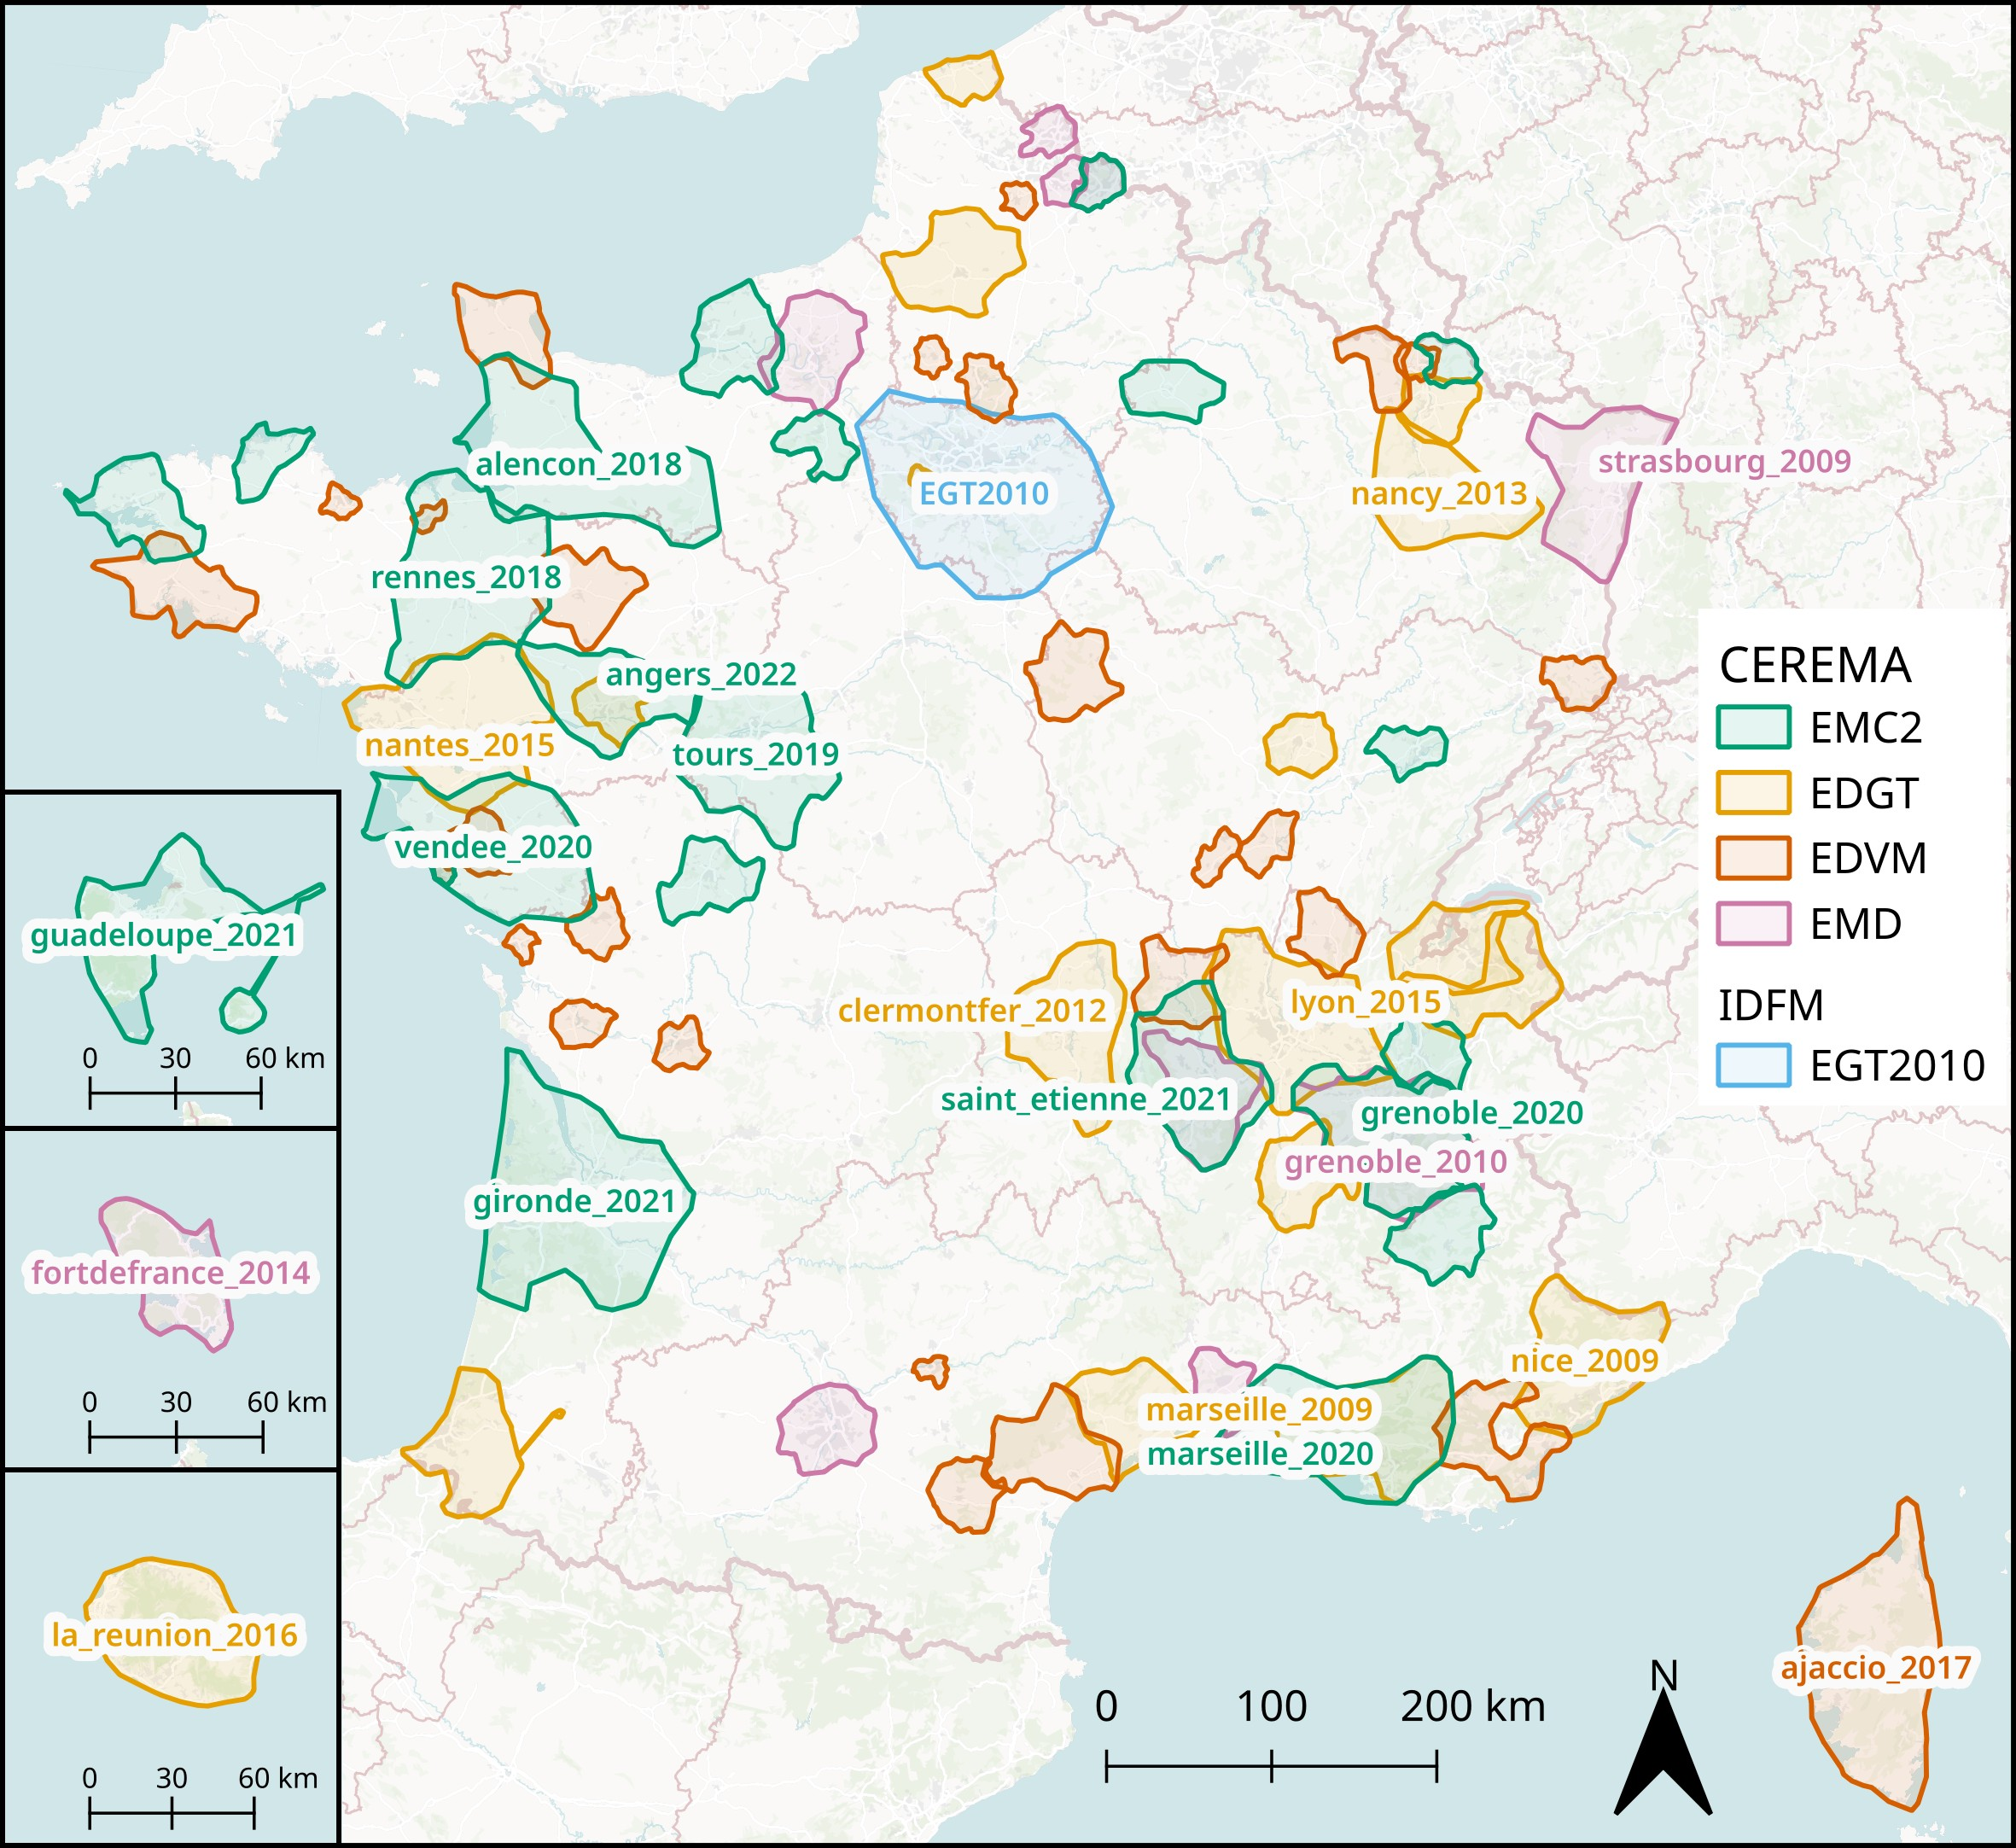
\includegraphics[width=0.6\textwidth]{../../output/maps/survey_map.jpg}
    \caption{Mobility surveys in France}
    \label{fig:survey_map}
    \footnotesize Note. This map shows the survey area for 78 surveys conducted between 2008 and 2022. Each color represents one of the 5 co-existing local survey formats, from CEREMA or Île-de-France Mobilités (IDFM).
\end{figure}

To address the challenges posed by fragmented mobility survey data in France, this study introduces MobiSurvStd, an open-source Python library designed to standardize diverse survey formats into a unified structure \citep{mobisurvstd_zenodo}.
Although this study focuses on intermodality, MobiSurvStd offers broader applications, enabling researchers and practitioners to analyze mobility behaviors across individual surveys or aggregated datasets.

The standardized format integrates 286 variables, organized across six key categories: households, persons, trips, legs, cars, and motorcycles.
Each variable is assigned a clearly defined data type and categorical variables include well-specified modalities to ensure consistency.
However, due to inherent differences in the original survey designs, not all variables or modalities are universally available across the entire dataset.

Overall, this comprehensive dataset of 78 surveys encompasses approximately \num{787000} surveyed individuals and includes information on roughly \num{2110000} trips.
For the analyses presented in this study, we focus exclusively on the subset of variables that are consistently available across all surveys.
These variables include individuals' age, gender, or professional occupation and trips' origin, destination, mode, purpose, distance.

To ensure the dataset accurately represents the entire French population, survey sample weights are recalibrated using key demographic and geographic variables.
The calibration process incorporated gender, age (divided into eight classes), professional occupation (divided into nine classes), and population density of home municipality (divided into three classes).
This recalibration is performed through margin calibration \citep{Deville1992,Icarus}.
The weighting adjustment is particularly important to address the under-representation of rural areas in the surveys.
All analysis and reported values in this study account for these recalibrated sample weights.


\section{Characterization of Intermodality}

\subsection{General Characteristics}

A trip represents a movement from an origin to a destination undertaken for a specific purpose, including work, school, shopping, or leisure activities.
Each trip may be composed of one or more legs, where a leg constitutes a continuous segment using a single mode of transportation.
For example, a home-to-work trip might consist of four sequential legs: driving to a parking facility, walking from the parking area to a nearby train station, traveling by train to a station near the workplace, and finally walking from that station to the final work destination.

This study defines \emph{intermodal trips} as those containing at least two legs using different transportation modes, excluding walking legs.
While many trips include short walking segments, these are not considered in the intermodal classification.

All public-transit modes, including buses, metros, and trains, are consolidated into a single ``public-transit'' category.
Consequently, trips combining different public transit modes, such as bus and train, are not classified as intermodal.
The mode categories considered in this analysis are car driver, car passenger, public transit, bicycle, and motorcycle.

This study focuses exclusively on ``local trips'', defined as trips with a Euclidean distance between origin and destination of less than \SI{80}{\kilo\meter}.
Longer trips, which typically involve different travel behaviors and modes such as high-speed trains or airplanes \citep{Tan2022}, are excluded from this analysis.
Additionally, when comparing intermodal and unimodal trips, walk-only trips are excluded, as these typically cover short distances where intermodality is not a practical alternative.

Within the dataset comprising 78 mobility surveys, there are \num{20310} intermodal trips, accounting for \SI{1.0}{\%} of all local trips.
However, these trips represent a disproportionately larger share of total travel distance, constituting \SI{3.7}{\%} of the total Euclidean distance traveled.
Intermodal trips exhibit significantly longer average distances (\SI{19.5}{\kilo\meter}) compared to unimodal trips (\SI{6.6}{\kilo\meter}).

Figure~\ref{fig:euclidean_dist_densities} illustrates the distribution of trip distances for both intermodal and unimodal trips.
The density plot reveals that intermodality is primarily used for trips exceeding \SI{5}{\kilo\meter} in length.
When focusing exclusively on trips longer than \SI{20}{\kilo\meter}, the share of intermodal trips increases substantially to \SI{6.5}{\%}.

\begin{figure}[htpb]
    \centering
    \includegraphics{../../output/paper_graphs/euclidean_dist_densities.pdf}
    \caption{Density distribution of trip distances by trip type}
    \label{fig:euclidean_dist_densities}
    \footnotesize Note. The density is estimated using kernel density estimation with a bandwidth factor of 0.03.
\end{figure}

Each trip recorded in the surveys includes information about the purpose at both the origin and destination.
We assign a single primary purpose to each trip by selecting the higher-ranked purpose based on the hierarchy established by \citet{Raux2018}: Work, Education, Escorting, Service, Shopping, and Leisure.
Figure~\ref{fig:purposes_bars} presents the distribution of trip purposes for both intermodal and unimodal trips.

The analysis reveals that work and education represent the dominant purposes for intermodal trips, accounting for \SI{78}{\%} of such trips.
In contrast, these purposes constitute only \SI{41}{\%} of unimodal trips.
While the cross-sectional nature of mobility surveys prevents direct observation of trip repetition, the predominance of work and education trips among intermodal journeys suggests that intermodality is primarily associated with regular, recurrent travel patterns.
This finding may also reflect the fact that work and education trips typically involve longer distances, which could make intermodal solutions more attractive or necessary.

\begin{figure}[htpb]
    \centering
    \includegraphics{../../output/paper_graphs/purposes_bars.pdf}
    \caption{Distribution of trip purposes by trip type}
    \label{fig:purposes_bars}
\end{figure}

Intermodal trips can involve different combinations of modes.
Figure~\ref{fig:intermodality_types_bars} illustrates the prevalence of different mode combinations among intermodal trips.
The data show a clear dominance of combinations involving public transit and cars.
Specifically, \SI{43.2}{\%} of intermodal trips combine public transit with traveling as a car passenger, while \SI{40.8}{\%} involve using public transit and driving a car.
These two categories together account for about \SI{85}{\%} of all intermodal trips.
Public transit also appears in the fourth most frequent combination, where it is used in conjunction with bicycle, representing \SI{5.3}{\%} of all intermodal trips.

Another notable combination involves using a car both as a driver and as a passenger during different segments of the same trip, accounting for \SI{6.6}{\%} of intermodal trips.
This pattern typically occurs in scenarios such as driving one's own vehicle to a ride-sharing meeting point and then continuing the journey as a passenger in another vehicle.
The remaining intermodal trips involve other combinations, including the use of motorcycles or the integration of more than two different modes.

\begin{figure}[htpb]
    \centering
    \includegraphics{../../output/paper_graphs/intermodality_types_bars.pdf}
    \caption{Distribution of mode combinations in intermodal trips}
    \label{fig:intermodality_types_bars}
\end{figure}

\subsection{Public transit and car combinations}

This subsection examines intermodal trips that integrate both public transit and car use, whether as a driver or passenger.
For short, in the remaining, we call these trips \emph{PT+Car}.

Figure~\ref{fig:pt_dist_ratio_density} presents the distribution of the share of Euclidean distance by public transit for \emph{PT+Car} trips.
The data reveal that public transit accounts for the majority of distance traveled in most cases.

On average, these intermodal trips involve \SI{17.0}{\kilo\meter} traveled by public transit compared to \SI{5.3}{\kilo\meter} by car.
This substantial difference indicates that cars primarily serve as an access mode to the public-transit network, particularly for individuals living beyond walking distance from transit stops.
The car segment effectively functions as a ``first-mile'' or ``last-mile'' solution, bridging the gap between origin or destination locations and the public transit system.

\begin{figure}[htpb]
    \centering
    \includegraphics{../../output/paper_graphs/pt_dist_ratio_density.pdf}
    \caption{Distribution of public-transit distance share in \emph{PT+Car} trips}
    \label{fig:pt_dist_ratio_density}
    \footnotesize Note. Walking distances are excluded from calculations. A \SI{50}{\%} share indicates equal distance traveled by public transit and by car.
\end{figure}

Demographic analysis reveals that individuals making trips combining public transit with car passenger status exhibit distinct characteristics.
A substantial \SI{81}{\%} of these travelers are either students or individuals without driving licenses, a proportion nearly three times higher than their \SI{21}{\%} representation among unimodal trip makers.
This significant overrepresentation can be attributed to the transportation constraints faced by these groups.
Students often lack access to personal vehicles, while individuals without driving licenses are legally prohibited from operating cars.
As a result, both demographic groups must depend on others to transport them to public-transit access points, particularly when these points are located at considerable distances from their origins.

The analysis of public-transit modes used in combination with cars reveals interesting insights into intermodal travel behavior.
We define the \emph{PT-Car transfer leg} as the public-transit leg immediately preceding or following the car leg in \emph{PT+Car} trips.
The \emph{transfer mode} refers specifically to the public-transit mode used during this PT-Car transfer leg.

Figure~\ref{fig:pt_modes_bars} illustrates the distribution of transfer modes used in \emph{PT+Car} trips.
The results show that trains (\SI{33}{\%}) and coaches (\SI{25}{\%}) are the predominant transfer modes.
In the French context, these modes typically serve as a connection between peripheral areas and urban centers.
However, their limited spatial coverage, with often only one train station per village or small town, necessitates the use of private vehicles to access these transit stops.


\begin{figure}[htpb]
    \centering
    \includegraphics{../../output/paper_graphs/pt_modes_bars.pdf}
    \caption{Distribution of public-transit transfer modes in \emph{PT+Car} trips}
    \label{fig:pt_modes_bars}
    \footnotesize Note. The chart displays the proportion of public-transit modes used during the transition between car and public-transit legs in either direction.
\end{figure}

Buses play a relatively minor role as transfer modes in \emph{PT+Car} trips, appearing in only \SI{13}{\%} of such trips.
This stands in contrast to the overall prominence of buses in public-transit usage, where they represent \SI{40}{\%} of all public-transit legs.
This indicates that car is more commonly used as an alternative to bus to reach major public-transit hubs, rather than being combined with bus services.

% A particularly notable finding is that, despite the generally long distances characteristic of intermodal trips, the public-transit component consists of a single leg in \SI{72}{\%} of \emph{PT+Car} trips.
% This suggests a preference for direct routes when using public transit in combination with car.

To analyze the spatial patterns of intermodal travel, this study employs the municipal classification system developed by INSEE, the French national statistics institute.
INSEE categorizes municipalities into three primary density classes: rural, intermediate-density, and dense.
To provide greater precision, we further subdivide the dense category using INSEE's definition of functional areas \emph{(aires d'attraction des villes)}.
This refinement allows us to distinguish between dense municipalities that serve as centers of their functional areas and those that do not.

We define the \emph{Car$\rightarrow$PT} trips as the \emph{PT+Car} trips where the car component comes before the public-transit component.
Table~\ref{tab:insee_density_flows} presents the distribution of \emph{Car$\rightarrow$PT} trips according to the density classification of both origin and destination municipalities.
The data reveal that \SI{70.5}{\%} of these intermodal trips originate from either intermediate-density or rural municipalities.
Moreover, a substantial majority (\SI{54.6}{\%}) of these trips terminate in dense municipalities that function as centers of their respective functional area.

\begin{table}[htpb]
    \centering
    \caption{Distribution of \emph{Car$\rightarrow$PT} trip flows by municipal density classification}
    \label{tab:insee_density_flows}
    \begin{tabular}{
            l
            S[detect-weight,mode=text,table-format=1.3]
            S[detect-weight,mode=text,table-format=1.3]
            S[detect-weight,mode=text,table-format=1.3]
            S[detect-weight,mode=text,table-format=1.3]
            S[detect-weight,mode=text,table-format=1.3]
        }
        \toprule
        Origin $\backslash$ Destination & {Center} & {Dense} & {Intermediate} & {Rural} & \textbf{Total origin}\\
        \colrule
        Center & 8.1 & 0.6 & 1.0 & 0.3 & \B 10.0 \\
        Dense & 13.1 & 5.2 & 0.9 & 0.3 & \B 19.5 \\
        Intermediate & 21.0 & 4.9 & 8.3 & 1.5 & \B 35.7 \\
        Rural & 12.4 & 2.6 & 10.7 & 9.0 & \B 34.8 \\
        \colrule
        \textbf{Total destination} & \B 54.6 & \B 13.4 & \B 20.9 & \B 11.1 & \B 100.0 \\
        \botrule
    \end{tabular}
    \flushleft\footnotesize Note. All values are expressed as percentages. The value of 21.0 in the third row indicates that \SI{21.0}{\%} of \emph{Car$\rightarrow$PT} trips originate in intermediate-density municipalities and terminate in dense municipalities that serve as center of their functional area.
\end{table}

Figure~\ref{fig:insee_density_flows_polar} provides a visual representation of these trip flows.
The diagram clearly illustrates that intermodality primarily facilitates travel from low-density or intermediate-density areas to high-density urban centers.
This pattern suggests that intermodal travel plays a crucial role in connecting peripheral areas with major urban hubs.

\begin{figure}[htpb]
    \centering
    \includegraphics{../../output/paper_graphs/insee_density_flows_polar.pdf}
    \caption{Spatial distribution of \emph{Car$\rightarrow$PT} trip flows by municipal density classification}
    \label{fig:insee_density_flows_polar}
    \footnotesize Note. The width of each arrow is proportional to the number of trips. Flows between municipalities of identical density categories are not displayed. Municipal density classifications follow INSEE's definitions of density and functional areas.
\end{figure}

\subsection{Analysis of Nearest Access Stop Selection}

This subsection examines the factors influencing travelers' choice of public-transit stops when transitioning between car and public transit modes.
% Understanding this decision-making process presents both methodological challenges and practical significance.
Such analysis can help predict traffic flows that could emerge with the development of new transit stops or the implementation of park-and-ride (P+R) facilities.
This investigation holds particular relevance in the French context, where the upcoming expansion of train stations with multimodal facilities through the Service Express Régional Métropolitain (SERM) initiative is expected to reshape regional transportation networks in the coming years.

This analysis also provides a methodological basis for modeling park-and-ride trips.
The potential applications of such modeling are demonstrated in the work of \citet{Yin2023}, who evaluate the effects of Paris's driving restriction zone policy.
They examine how people might use park-and-ride facilities to reach restricted areas without driving inside the zone.
Their model assumes that park-and-ride users would drive to the nearest transit stop from their starting point.
This nearest-stop assumption offers a reference point for comparing with the empirical findings presented in this study.

The mobility surveys used in this study present certain methodological limitations regarding spatial precision.
Rather than providing exact coordinates for origins, destinations, and selected stops, the surveys locate these points within predefined zones.
These zones vary in size, with an average area of approximately \SI{6}{\kilo\meter\squared}.
The Île-de-France survey represents an exception, employing a finer grid system of \SI{100}{\meter} by \SI{100}{\meter}, resulting in zones of \SI{0.01}{\kilo\meter\squared}.

To supplement the survey data, this analysis incorporates comprehensive information on public-transit stop locations.
These data were compiled by processing 461 General Transit Feed Specification (GTFS) files covering the entire French territory.%
\footnote{These GTFS files were collected from \url{https://transport.data.gouv.fr/}.}
For the year 2025, the dataset identifies all public-transit stops served by at least one transit line, categorizing each stop by the mode it is served by, including train, tram, metro.

This analysis focuses on \emph{Car$\rightarrow$PT} trips where the first public-transit mode used is either train, tram, or metro.
Our comprehensive public-transit stops database contains 1453 train stops, 602 tram stops, and 464 metro stops.
For this analysis, we define \emph{access zone} as the survey zones where travelers transfer transition from car to public transit.

Within each access zone, we identify all relevant transit stops corresponding to the reported transfer mode.
For approximately \SI{8}{\%} of eligible trips, there is no stop that matches the reported transfer mode within the access zone, or within 50 meters of it.
This discrepancy may result from either incomplete stop data in our database or potential reporting errors by survey respondents regarding their access zone or transit mode.
These trips with missing stop information are excluded from further analysis.

Figure~\ref{fig:nearest_stop_zones} illustrates an example of a valid trip included in our analysis.
This example shows a trip where the traveler accessed the public-transit network by train, with a train station clearly located within the designated access zone.

\begin{figure}[htpb]
    \centering
    \includegraphics{../../output/maps/nearest_stop_zones.jpg}
    \caption{Example of origin and access zones for a trip with train as transfer mode}
    \label{fig:nearest_stop_zones}
    \footnotesize Note. The access zone (orange) is adjacent to the origin zone (blue).
    A single train station is located within the access zone, with additional train stations located near the origin zone.
\end{figure}

To determine whether travelers use the closest stop to their origin, we employ a geometric approach that accounts for the zonal structure of our data.
Since the exact origin location within each zone is unknown, we cannot directly identify the closest stop.
Instead, we examine each vertex of the origin zone to determine the nearest stop.

When the closest stop for all vertices of the origin zone lies within the access zone, we conclude with confidence that the traveler used the nearest stop to their origin.
Conversely, when the closest stop for all vertices is outside the access zone, we can confidently determine that the traveler did not use the nearest stop.
For cases where some vertices have the closest stop inside the access zone and others have it outside, we cannot definitively determine whether the traveler used the nearest stop.

Figure~\ref{fig:nearest_stop_example} illustrates a scenario where this determination cannot be made.
The location of the nearest station depends on the exact origin point within the zone: the station within the access zone is closest to the green dot, while the station outside the access zone is closest to the orange dot.

\begin{figure}[htpb]
    \centering
    \includegraphics{../../output/maps/nearest_stop_example_wctr.jpg}
    \caption{Ambiguity in determining nearest station for an example trip}
    \label{fig:nearest_stop_example}
    \footnotesize Note. The nearest station depends on the exact origin location within the zone.
    If the traveler's origin is located at the green dot, then the station within the access zone is indeed the closest.
    If however the traveler's origin is located at the orange dot, then the closest station is outside the access zone.
\end{figure}

Table~\ref{tab:nearest} presents the results of this analysis for train, tram, and metro access modes over all eligible \emph{Car$\rightarrow$PT} trips.
For train access, we can definitively determine that travelers used the closest stop in \SI{37.0}{\%} of cases and did not use the closest stop in \SI{32.7}{\%} of cases.
For the remaining \SI{30.3}{\%} of trips, we cannot make a definitive determination.
However, given the relatively small size of the zones, it is reasonable to assume that in these ambiguous cases, travelers likely used either the closest stop or one very near to it.
These findings align with the analysis of park-and-ride in Minneapolis by \citet{Webb2020}.
They find that \SI{49}{\%} of surveyed users selected the park-and-ride facility that minimizes their driving time from origin.

\begin{table}[htpb]
    \centering
    \caption{Share of \emph{Car$\rightarrow$PT} trips using the closest stop from origin by access mode}
    \label{tab:nearest}
    \begin{tabular}{lccc}
        \toprule
         & Train & Tram & Metro \\
         \colrule
        Definitely uses closest stop & 37.0 & 9.0 & 21.3 \\
        Definitely does not use closest stop & 32.7 & 64.7 & 57.1 \\
        Indeterminate & 30.3 & 26.2 & 21.6 \\
        \botrule
    \end{tabular}
    \flushleft\footnotesize Note. All values represent percentage. For train access, \SI{37.0}{\%} of trips definitely used the closest stop, i.e., the closest train stop from all vertices of the origin zone are within the access zone.
\end{table}

In contrast to train access, our findings indicate that travelers typically do not use the closest stop for tram (\SI{64.7}{\%}) and metro (\SI{57.1}{\%}) access.
Several factors may influence the choice of a different stop.
Travelers might choose a stop that offers a more direct route to their destination rather than selecting the geographically closest stop, which might imply traveling in the opposite direction initially.
The decision to bypass the nearest stop may reflect a preference for transit lines that offer better service frequency or more convenient transfers to reach the ultimate destination.

The quality of park-and-ride facilities might also play a significant role in stop selection.
Factors such as the number of available parking spaces and the walking distance between parking areas and transit platforms can influence travelers' choices.

Finally, it is important to note that our analysis uses Euclidean distance to determine the closest stop, which represents a simplification of actual travel behavior.
A more refined approach would consider actual travel time by car from the origin to potential access stops.
The stop with the shortest travel time might differ from the geographically closest stop due to factors such as traffic congestion or the specific layout of the road network.

\section{Conclusion}

This study provides new empirical insights into intermodal travel patterns in France by leveraging a harmonized dataset of 78 mobility surveys.
The findings reveal that intermodal trips are characterized by long distances, averaging \SI{19.5}{\kilo\meter}, with the combination of car and public transit representing the dominant pattern (\SI{85}{\%} of intermodal trips).
The data show that car primarily serve as access mode to public transit in low-density areas, where travelers typically complete the majority of their journey using public transit.
While proximity to origin strongly determines train stop choice, this factor is less relevant for trams and metro, suggesting that service quality and network connectivity play crucial roles.

These results offer guidance for transportation planners seeking to design more effective multimodal systems, particularly in the context of France's ongoing SERM infrastructure development.
Through the development and application of the MobiSurvStd harmonization framework, this research establishes a methodological foundation for future investigations of complex and less common mobility behaviors.

\section*{Acknowledgements}

This work has benefited from invaluable advise and feedback from Gabrielle Gambuli, Jimmy Argmoogum, André de Palma, Tatiana Seregina, and Laura Echeverri-Guzman.
Any errors or omissions that may remain are the sole responsibility of the author.

% Acknowledgements and Reference heading should be left justified, bold, with the first letter capitalized but have no numbers. Text below continues as normal.

%% The Appendices part is started with the command \appendix;
%% appendix sections are then done as normal sections
%% \appendix

%% \section{}
%% \label{}

% \appendix
% \section{An example appendix}
% Authors including an appendix section should do so before References section. Multiple appendices should all have headings in the style used above. They will automatically be ordered A, B, C etc.

% \subsection{Example of a sub-heading within an appendix}
% There is also the option to include a subheading within the Appendix if you wish.
%% References
%%
%% Following citation commands can be used in the body text:
%% Usage of \cite is as follows:
%%   \cite{key}         ==>>  [#]
%%   \cite[chap. 2]{key} ==>> [#, chap. 2]
%%

%The citation must be used in following style: \cite{article-minimal} \cite{article-full} \cite{article-crossref} \cite{whole-journal}.
%% References with BibTeX database:

\bibliography{bibliography}
\bibliographystyle{elsarticle-harv}


%% Authors are advised to use a BibTeX database file for their reference list.
%% The provided style file elsarticle-num.bst formats references in the required Procedia style

%% For references without a BibTeX database:

% \begin{thebibliography}{}

% %% \bibitem must have the following form:
% %%   \bibitem{key}...
% %%

% % \bibitem[Clark et al.(1962)]{clark}Clark, T., Woodley, R., De Halas, D., 1962. Gas-Graphite Systems, in ``{\it Nuclear Graphite}''.
% % In: Nightingale, R. (Ed.). Academic Press, New York, pp. 387.

% % \bibitem[Deal and Grove(2009) ]{Deal}Deal, B., Grove, A., 1965. General Relationship for the Thermal Oxidation of Silicon. Journal of Applied Physics 36.2, 37--70.

% % \bibitem[Deep(2009)]{Deep}Deep-Burn Project: Annual Report for 2009, Idaho National Laboratory, Sept. 2009.

% % \bibitem[Fachinger(2004)]{Fachinger2004}Fachinger, J., den Exter, M., Grambow, B., Holgerson, S., Landesmann, C., Titov, M., Podruhzina, T., 2004. ``Behavior of spent HTR fuel elements in aquatic phases of repository host rock formations,'' 2nd International Topical Meeting on High Temperature Reactor Technology. Beijing, China, paper \#B08.

% % \bibitem[Fachinger(2006)]{Fachinger2006}Fachinger, J., 2006. Behavior
% % of HTR Fuel Elements in Aquatic Phases of Repository Host Rock Formations. Nuclear Engineering \& Design 236.3,      54.

% \end{thebibliography}

\clearpage

%%%% This page is for instructions only, once the article is finalize please omit the below text before creating the final PDF
% \normalMode

% \section*{Instructions to Authors for LaTeX template:}

% \section{ZIP mode for LaTeX template:}

% The zip package is created as per the guide lines present on the URL http://www.elsevier.com/author-schemas/ preparing-crc-journal-articles-with-latex for creating the LaTeX zip file of Procedia LaTeX template.  The zip generally contains the following files:
% \begin{Itemize}[]\leftskip-17.7pt\labelsep3.3pt
% \item ecrc.sty
% \item  elsarticle.cls
% \item elsdoc.pdf
% \item .bst file
% \item Manuscript templates for use with these bibliographic styles
% \item  Generic and journal specific logos, etc.
% \end{Itemize}

% The LaTeX package is the main LaTeX template. All LaTeX support files are required for LaTeX pdf generation from the LaTeX template package.

% {\bf Reference style .bst file used for collaboration support:} In the LaTeX template packages of all Procedia titles a new ``.bst'' file is used which supports collaborations downloaded from the path http://www.elsevier.com/author-schemas/the-elsarticle-latex-document-class

\end{document}

%%
%% End of file.
